In this project we investigate a fermionic system of N=2, 6 and 12 electrons. It is a so-called closed shell-system. The Hamiltonian used to model this system is

\begin{equation}
\label{eq:finalH}
\hat{H}=\sum_{i=1}^{N} \left(  -\frac{1}{2} \nabla_i^2 + \frac{1}{2} \omega^2r_i^2  \right)+\sum_{i<j}\frac{1}{r_{ij}},
\end{equation}
where 
$$\hat{H}_0=\sum_{i=1}^{N} \left(  -\frac{1}{2} \nabla_i^2 + \frac{1}{2} \omega^2r_i^2  \right)$$
is the single particle part and

\begin{equation}\label{eq:hamilton_interaction}
\hat{H}_1=\sum_{i<j}\frac{1}{r_{ij}},
\end{equation}

represent the interaction potential between particles. The Hamiltonian is written in atomic units, which implies that $\hbar = 1, m= 1$, the unit of length is $a_0 = ...$ and the unit of energy is $...$.  We also have $r_{ij}=\vert \bm{r}_i-\bm{r}_j\vert= \sqrt{(x_i-x_j)^2 + (y_i-y_j)^2}$ and $\omega$ is the oscillator frequency. Later we will study the dependence of the system on the oscillator frequency. 

\subsection{Two particle system}

The single particle wave function in two dimensions is
\begin{equation}\label{eq:single_particle_wf}
\phi_{n_x,n_y}(x,y) = A H_{n_x}(\sqrt{\omega}x)H_{n_y}(\sqrt{\omega}y)\exp{(-\omega(x^2+y^2)/2}.
\end{equation}
where the functions $H_{n_x}(\sqrt{\omega}x)$ are Hermite polynomials,  while $A$ is a normalization constant. The relevant Hermite polynomials in this project are listed in Appendix \ref{app:hermite_and_derivatives}. $\omega$ is the trap frequency.

For the lowest-lying state, $E_{00}$  (see Fig. \ref{fig:states}), we have $n_x=n_y=0$ and an energy $\epsilon_{n_x,n_y}=\omega(n_x+n_y+1) = \omega$, the total energy of the lowest-lying state is hence $2\omega$ because there is room for two electrons with opposite spins. 

\begin{figure}[H]
\center
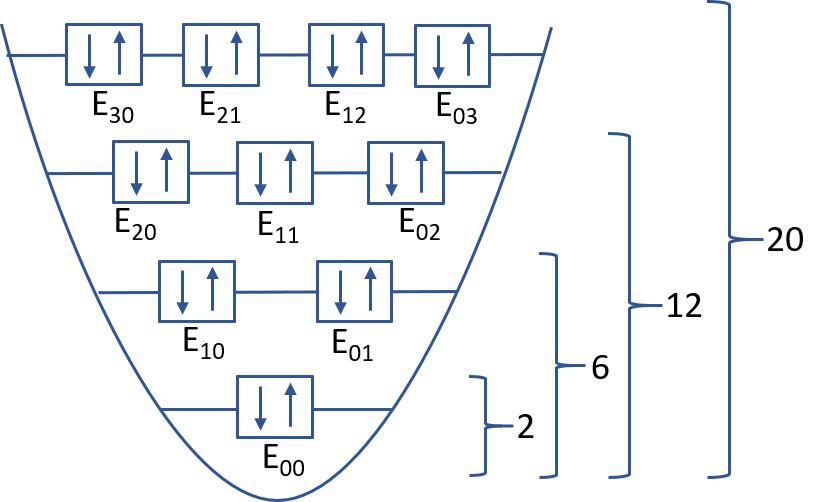
\includegraphics[width=0.6\linewidth]{../Results/states}\caption{•}\label{fig:states}
\end{figure}

The expectation value can be found by solving the equation

\begin{equation}\label{eq:expectation_energy}
   \langle E \rangle =
   \frac{\int d\bm{r}_1d\bm{r}_2\psi^{\ast}_T(\bm{r}_1,\bm{r}_2)\hat{H}(\bm{r}_1,\bm{r}_2)\psi_T(\bm{r}_1,\bm{r}_2)}
        {\int d\bm{r}_1d\bm{r}_2\psi^{\ast}_T(\bm{r}_1,\bm{r}_2)\psi_T(\bm{r}_1,\bm{r}_2)}.
\end{equation}

We will use Variational Monte Carlo (VMC) methods to evaluate the Eq. \ref{eq:expectation_energy} \cite{project1}. The exact wave function for two not interacting electrons in the ground state is given by

\begin{equation*}
\Phi(\bm{r}_1,\bm{r}_2) = C\exp{\left(-\omega(r_1^2+r_2^2)/2\right)},
\end{equation*}

where $r_i = \sqrt{x_i^2+y_i^2}$ and C is a normalization constant. The trial wavefunction we use for the not interacting case is 
\begin{equation*}
\Phi(\bm{r}_1,\bm{r}_2) = C\exp{\left(-\alpha\omega(r_1^2+r_2^2)/2\right)}.
\end{equation*}

with the parameter $\alpha$. From the exact wave function we know that $\alpha = 1$ for the situation without interaction. On the other hand, for the interacting case, the trial wave function for the two-electron system is

\begin{equation}
   \psi_{T}(\bm{r}_1,\bm{r}_2) = 
   C\exp{\left(-\alpha\omega(r_1^2+r_2^2)/2\right)}
   \exp{\left(\frac{ar_{12}}{(1+\beta r_{12})}\right)}, 
\label{eq:trial_interacting}
\end{equation}

where we introduce another parameter, $\beta$, and a spin factor, $a$. $a$ is 1 when the two electrons have anti-parallel spins and $1/3$ when they have the parallel spins (this is not relevant before we introduce more particles to the system, as can be seen from Fig. \ref{fig:states}).

\subsection{More particles}

Since we are looking at closed shell systems, the next amount of particles are six. We can see this from Fig. \ref{fig:states}, there are room for two electrons with opposite spin in two different states, in addition to the two in the lowest lying state. The trial wave function is now given by

\begin{equation}
   \psi_{T}(\bm{r}_1,\bm{r}_2,\dots, \bm{r}_6) = 
   Det\left(\phi_{1}(\bm{r}_1),\phi_{2}(\bm{r}_2),
   \dots,\phi_{6}(\bm{r}_6)\right)
   \prod_{i<j}^{6}\exp{\left(\frac{a r_{ij}}{(1+\beta r_{ij})}\right)},
\end{equation}

where 
$$ Det\left(\phi_{1}(\bm{r}_1),\phi_{2}(\bm{r}_2),
   \dots,\phi_{6}(\bm{r}_6)\right) =  \begin{vmatrix}
  \phi_{1}(\bm{r}_1) & \phi_{2}(\bm{r}_1) & \cdots & \phi_{6}(\bm{r}_1) \\
  \phi_{1}(\bm{r}_2) & \phi_{2}(\bm{r}_2) & \cdots & \phi_{6}(\bm{r}_2) \\
  \vdots  & \vdots  & \ddots & \vdots  \\
  \phi_{1}(\bm{r}_6) & \phi_{2}(\bm{r}_6) & \cdots & \phi_{6}(\bm{r}_6) 
\end{vmatrix}$$
is the Slater determinant. This determinant occurs because electron are indistinguishable particles and they are antisymmetric ... . The functions, $\phi_{i}(\bm{r}_j)$,  are given by Eq. \ref{eq:single_particle_wf} and the notation is explained in Tab. \ref{tab:notation_wavefunctions}. 

\begin{table}[H]\caption{The relation between the notation used in the determinant (left) compared to Eq. \ref{eq:single_particle_wf} (right). }\label{tab:notation_wavefunctions}
\large
\center
\begin{tabular}{l|l} 
$\phi_{1}$ & $\phi_{n_x=0, n_y=0}$\\
$\phi_{2}$ & $\phi_{n_x=0, n_y=0}$\\
$\phi_{3}$ & $\phi_{n_x=1, n_y=0}$\\
$\phi_{4}$ & $\phi_{n_x=1, n_y=0}$\\
$\phi_{5}$ & $\phi_{n_x=0, n_y=1}$\\
$\phi_{6}$ & $\phi_{n_x=0, n_y=1}$\\
\end{tabular}
\begin{tabular}{c}
$\,$
\end{tabular}
\begin{tabular}{l|l} 
$\phi_{7}$ & $\phi_{n_x=2, n_y=0}$\\
$\phi_{8}$ & $\phi_{n_x=2, n_y=0}$\\
$\phi_{9}$ & $\phi_{n_x=1, n_y=1}$\\
$\phi_{10}$ & $\phi_{n_x=1, n_y=1}$\\
$\phi_{11}$ & $\phi_{n_x=0, n_y=2}$\\
$\phi_{12}$ & $\phi_{n_x=0, n_y=2}$\\
\end{tabular}
\end{table}

Similarly if we include another "shell" in our system we get 12 particles and the trial wavefunction is 

\begin{equation}
   \psi_{T}(\bm{r}_1,\bm{r}_2, \dots,\bm{r}_{12}) = 
   Det\left(\phi_{1}(\bm{r}_1),\phi_{2}(\bm{r}_2),
   \dots,\phi_{12}(\bm{r}_{12})\right)
   \prod_{i<j}^{12}\exp{\left(\frac{ar_{ij}}{(1+\beta r_{ij})}\right)}.
\end{equation}

The determinant have the same structure as for six particles and the relation to the single-particle wave functions are shown in Tab. \ref{tab:notation_wavefunctions}.

\subsection{One-body density}

The radial one-body density is a measure of the spactial distribution of the electrons with respect to the distance from the middle of the harmonic oscillator trap. To calculate the radial one-body density, we want to sample the position of the electrons. The distance from the origin to a set cut-off is seperated into bins with a length $\Delta r$. For every Monte Carlo step, the distance between the electron's position and the origin is calculated, and the bin that corresponds to the current distance get a count. In the end, you have an array corresponding to the different bins with counts corresponding to how many times an electron was found to have that particular distance to the origin. This array is normalized by dividing by the number of Monte Carlo steps. However, to get the density, we have to divide the number in the bins with the area or volume the bin represents. Because we have two-dimensional problem in this project and we calculate the radial one-body density, we devide bin $i$ with the area $ A = \pi (r_i+\Delta r)^2 - \pi r_i^2$ where $r_i$ is distance from the origin to bin $i$. \textit{normalized to the number of particles. Mention. Should happen automatically... Does not happen automatically for me, but I have notice that Even has the same scale on the y-axis.}\cite{Evens_master}

\subsection{Virial theorem}

The virial theorem gives a relation between the time-average total kinetic energy, $\left<T\right>$, and the time-average external potential energy, $\left<V_{ext}\right>$, that is

\begin{equation}\label{eq:virial_theorem}
2\left< T\right> = n\left< V_{ext}\right>
\end{equation}

where $V(r) = Br^n$. In our case when we do not include interaction $n = 2$ from the external potential term in Eq. \ref{eq:finalH}, and therefore the average kinetic energy should be equal to the average potential energy. This can be used as a test to see if the simulations executed are correct. 

\subsection{Trap frequency}

The trap frequency changes the external potential felt by the electrons. Figure \ref{fig:harmonic_oscillator_potential} shows how a larger trap frquency, $\omega$, results in a narrower external potential. In this narrow harmonic oscillator trap, the electrons are forced to be closer to eachother. Later, we will investigate how $\omega$ affects the energy when the electrons are interacting with eachother through the potential given in Eq. \ref{eq:hamilton_interaction}

\begin{figure}[H]
\center
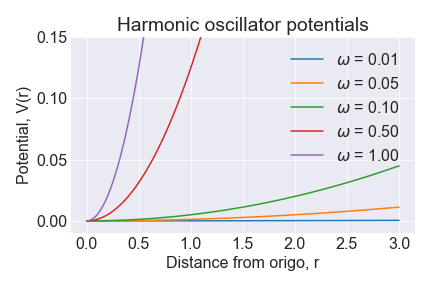
\includegraphics[width=0.5\linewidth]{../Results/harmonic_oscialltor_potentials}\caption{•}\label{fig:harmonic_oscillator_potential}
\end{figure}
